\subsection{ボリュームを使って画像を動かしてみよう}
A0にボリューム(\#104)をつなげてみましょう。HSPスクリプトエディタで/home/pi/ome/05/angle.hspを開いて実行してください。\\

\begin{lstlisting}[caption=angle.hsp,label=angle.hsp]
#include "hsp3dish.as"
#include "rpz-gpio.as"

celload("hyou.png"),2
p = 50

spiopen 0

*main
	data = spiget(0,0)
	p = rasp_map(data, 0, 1023, 0, 440)

	redraw 0
	pos 100,100
	mes data
	mes p
	pos 0,0
	celput 2
	redraw 1

	wait 10	
	goto *main

spiclose 0
\end{lstlisting}

画像を使うためには\code{celload}命令を使います。
\code{celload (“画像の名前”),画像の番号}
で画像を読み込むことができます。読み込んだ画像は\code{celput 画像の番号}で表示することができます。画像や文字の位置は\code{pos}命令を使って決めることができます。\code{pos}命令で画像の位置がどう変わるのか、 図\ref{angle.hsp}を見てみましょう。

\begin{figure}[H]
\centering
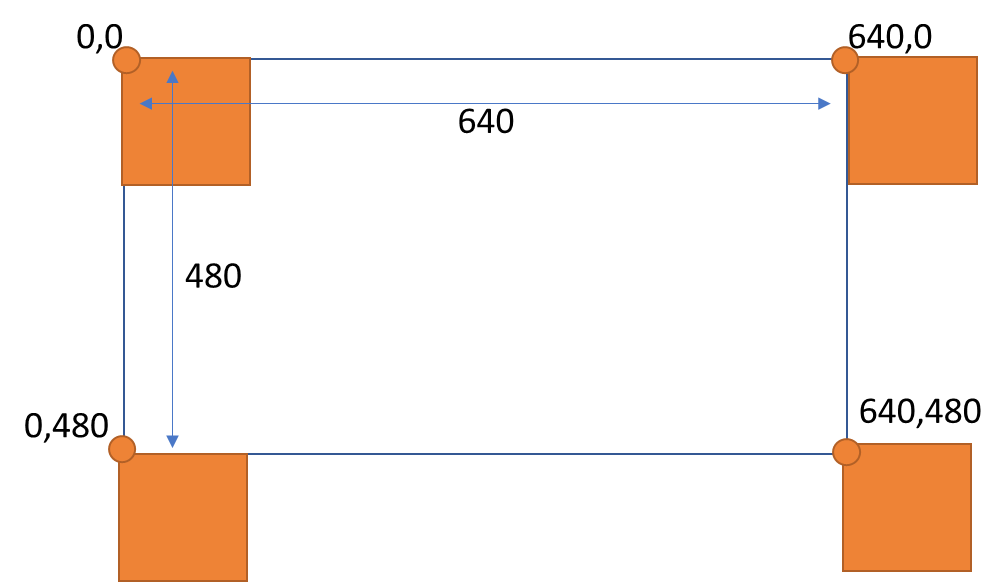
\includegraphics[scale=0.8]{images/chap05/text05-img034.png}
\caption{画面と位置のかんけい}
\label{angle.hsp}
\end{figure}

みなさんが使っているHSPでは画面の横のサイズは640、縦のサイズは480で表示されています。青い四角が画面、オレンジの四角が画像だと思ってください。画像や文字の位置は\code{pos 横の位置,縦の位置}を使って決めます。横の位置は一番左からどれくらい離れているか、縦の位置は一番上からどれくらい離れているかで決まります。例えば左上は0,0と書くことができます。右下は640,480と書くことができます。一番右上に画像を表示したいとき、640,0と書いてしまうと画像がディスプレイからはみ出てしまいます。\code{pos}命令では画像の左上の点をどこに置くか指定しているからです。画像をディスプレイの中にいれたいときは、画像のサイズ分だけ\code{pos}で指定する位置を左にずらさないといけません。\\

\begin{tcolorbox}[title=\useOmetoi]
\begin{enumerate}
\item ボリューム(\#104)をA0につなげて/home/pi/ome/05/block3\_angle.hspを実行してみましょう。ボリューム(\#104)を使ってブロック崩しを遊ぶことができます。
\end{enumerate}
\end{tcolorbox}
\begin{tcolorbox}[title=\useOmetoi]
\begin{enumerate}
\item angle.hspの pos 0,0 の数字を変えて、右上に画像を表示しましょう。(だいたいで良いです)
\end{enumerate}
\end{tcolorbox}
\begin{tcolorbox}[title=\useOmetoi]
\begin{enumerate}
\item angle.hspの pos 0,0 の数字を変えて、真ん中に画像を表示しましょう。(だいたいで良いです)
\end{enumerate}
\end{tcolorbox}
\begin{tcolorbox}[title=\useOmetoi]
\begin{enumerate}
\item angle.hspの pos 0,0 の数字を変えて、左下に画像を表示しましょう。(だいたいで良いです)
\end{enumerate}
\end{tcolorbox}
\begin{tcolorbox}[title=\useOmetoi]
\begin{enumerate}
\item angle.hspの pos 0,0 の数字を変えて、右下に画像を表示しましょう。(だいたいで良いです)
\end{enumerate}
\end{tcolorbox}
\begin{tcolorbox}[title=\useOmetoi]
\begin{enumerate}
\item ボリュームを使って画像を横に動かしてみましょう。angle.hspの\code{pos 0,0}を\code{pos p,0}に変えて実行してください。
\end{enumerate}
\end{tcolorbox}
\begin{tcolorbox}[title=\useOmetoiAlpha]
\begin{enumerate}
\item 前の問題では、ボリュームの値を大きくすると、ヒョウが右に動きます。ボリュームの入力はdata = spiget(0,0)で受け取り、p = rasp\_map(data, 0, 1023, 0, 440)で値を0~440に変換します。ボリュームの値で画像を右に動かすには、変数を使います。pには0~440の値が入るため、pos命令で横をpにすればボリュームの値で右に動かすことができます。\\
時間があったら挑戦してみましょう。ボリュームの値を大きくしていくと、画像が右から左に動くようにプログラムを変えましょう。
\end{enumerate}
\end{tcolorbox}
\begin{tcolorbox}[title=\useOmetoiAlpha]
\begin{enumerate}
\item 時間があったら挑戦してみましょう。ボリュームの値で画像が縦に動くようにプログラムを変えましょう。
\end{enumerate}
\end{tcolorbox}